% =============================================================================
% CHO MarketWatch : Plateforme Intelligente de Suivi et Pilotage des Prix en Temps Réel
% =============================================================================

\documentclass[12pt,a4paper,oneside]{report}

% --- Encodage et langue ---
\usepackage[utf8]{inputenc}
\usepackage[T1]{fontenc}
\usepackage[french]{babel}
\usepackage{lmodern}
\usepackage{microtype}

% --- Mise en page ---
\usepackage{geometry}
\geometry{top=2.5cm,bottom=2.5cm,left=3cm,right=2.5cm}
\usepackage{setspace}
\setstretch{1.2}

% --- Utilitaires ---
\usepackage{graphicx}
\graphicspath{{figures/}}
\usepackage{xcolor}
\usepackage{array}
\usepackage{booktabs}
\usepackage{longtable}
\usepackage{float}
\usepackage{enumitem}
\usepackage{caption}
\usepackage{hyperref}
\usepackage{fancyhdr}
\usepackage{listings}
\usepackage{tikz}

% --- Couleurs ---
\definecolor{codegray}{rgb}{0.40, 0.40, 0.40}
\definecolor{codeblue}{rgb}{0.10, 0.24, 0.46}
\definecolor{codegreen}{rgb}{0.20, 0.45, 0.30}
\definecolor{codebg}{rgb}{0.96, 0.96, 0.96}

% --- Style de code ---
\lstdefinestyle{choStyle}{
	basicstyle=\ttfamily\small,
	backgroundcolor=\color{codebg},
	keywordstyle=\color{codeblue}\bfseries,
	commentstyle=\color{codegreen},
	stringstyle=\color{red!60!black},
	numberstyle=\tiny\color{codegray},
	numbers=left,
	numbersep=8pt,
	breaklines=true,
	showstringspaces=false,
	frame=single
}
\lstset{style=choStyle}

% --- Identite du projet ---
\newcommand{\ProjectName}{CHO MarketWatch}
\newcommand{\ProjectOfficialTitle}{CHO MarketWatch : Plateforme Intelligente de Suivi et Pilotage des Prix en Temps Réel}

% --- Entete et pied de page ---
\pagestyle{fancy}
\fancyhf{}
\fancyhead[L]{\nouppercase{\leftmark}}
\fancyhead[R]{\ProjectName}
\fancyfoot[C]{\thepage}
\setlength{\headheight}{15pt}
\renewcommand{\headrulewidth}{0.4pt}
\renewcommand{\footrulewidth}{0.0pt}

% --- Liens ---
\hypersetup{
	colorlinks=true,
	linkcolor=codeblue,
	citecolor=codeblue,
	urlcolor=codeblue
}

% --- Noms des elements ---
\renewcommand{\contentsname}{Table des matieres}
\renewcommand{\listfigurename}{Liste des figures}
\renewcommand{\listtablename}{Liste des tableaux}

% --- Macro placeholder pour les figures ---
\newcommand{\figureplaceholder}[3][6cm]{%
\begin{figure}[H]
\centering
\fbox{\parbox[c][#1][c]{0.90\textwidth}{\centering\textbf{Placeholder image}\\#2}}
\caption{#3}
\end{figure}
}

% =============================================================================
% DOCUMENT
% =============================================================================
\begin{document}

% --- Page de garde ---
\pagenumbering{gobble}
\begin{titlepage}
\thispagestyle{empty}

\begin{center}
\begin{minipage}[t]{0.36\textwidth}
\vspace{0pt}
\centering
{\scriptsize \textbf{\mbox{R\'epublique Tunisienne}}}\\
{\scriptsize \textbf{\mbox{Minist\`ere de l'Enseignement Sup\'erieur}}}\\
{\scriptsize \textbf{\mbox{et de la Recherche Scientifique}}}
\end{minipage}
\hfill
\begin{minipage}[t]{0.20\textwidth}
\vspace{0pt}
\centering

\includegraphics[width=2.55cm]{university_logo.png}
\end{minipage}
\hfill
\begin{minipage}[t]{0.36\textwidth}
\vspace{0pt}
\centering
{\scriptsize \textbf{\mbox{Universit\'e de Sfax}}}\\
{\scriptsize \textbf{\mbox{Institut Sup\'erieur d'Administration}}}\\
{\scriptsize \textbf{\mbox{des Affaires}}}
\end{minipage}

\vspace{2.2cm}

{\fontsize{28}{34}\selectfont \textbf{Projet de fin d'\'etudes}}\\[0.9cm]
{\Large \textbf{En vue de l'obtention du dipl\^ome de Licence en Informatique de Gestion}}\\[0.45cm]
{\Large \textbf{Parcours : Business Intelligence}}\\[1.7cm]

\begin{tikzpicture}
\node[
	draw=black,
	rounded corners=22pt,
	line width=1.4pt,
	minimum width=0.80\textwidth,
	minimum height=4.5cm,
	align=center,
	inner sep=14pt
] {
	\parbox{0.66\textwidth}{\centering\LARGE\textbf{\ProjectOfficialTitle}}
};
\end{tikzpicture}

\vfill

\begin{minipage}[t]{0.42\textwidth}
\vspace{0pt}
\raggedright
\textbf{Pr\'esent\'e par :}\\[0.70cm]
Khalil Amamri\\
Mahdi ElhadjAmor
\end{minipage}
\hfill
\begin{minipage}[t]{0.42\textwidth}
\vspace{0pt}
\raggedright
\textbf{Dirig\'e par :}\\[0.70cm]
M. Mazouzi Mohamed (Encadrant acad\'emique)\\
M. Elloumi Amine (Encadrant professionnel)
\end{minipage}

\vspace{1.8cm}
{\Large Ann\'ee universitaire 2025 - 2026}
\end{center}

\end{titlepage}
\clearpage


% --- Pages preliminaires ---
\pagenumbering{roman}
\setcounter{page}{1}
\chapter*{Remerciements}
\addcontentsline{toc}{chapter}{Remerciements}

Nous tenons a remercier toutes les personnes qui nous ont aides a realiser ce projet.

Nous adressons nos sincres remerciements a notre encadrant pour son accompagnement, ses remarques techniques et son suivi regulier pendant toutes les phases du travail.

Nous remercions egalement l'equipe de CHO Company pour sa confiance, sa disponibilite et l'acces aux besoins metier qui ont permis de construire une solution utile et realiste.

Nous remercions enfin nos enseignants, nos familles et nos proches pour leur soutien moral et leurs encouragements tout au long de notre parcours.

\clearpage


\tableofcontents
\clearpage

\listoffigures
\clearpage

\listoftables
\clearpage

% --- Corps du rapport ---
\pagenumbering{arabic}

\chapter*{Introduction générale}
\addcontentsline{toc}{chapter}{Introduction générale}

Dans un environnement économique caractérisé par une concurrence accrue et des fluctuations fréquentes des prix, les entreprises doivent s'appuyer sur des données fiables et actualisées afin de prendre des décisions stratégiques pertinentes.

Le groupe \textbf{CHO}, acteur majeur dans le secteur de l'huile d'olive, opère sur plusieurs marchés internationaux où le suivi des prix constitue un levier essentiel de compétitivité. En effet, la diversité des marchés, la multiplicité des concurrents et la variabilité des prix rendent la surveillance des données particulièrement complexe.

Actuellement, le processus de collecte et d'analyse des prix repose en grande partie sur des méthodes manuelles, notamment la collecte terrain et l'utilisation de fichiers Excel. Cette approche présente plusieurs limites, notamment en termes de fiabilité, de rapidité et d'exploitation des données.

Dans ce contexte, la problématique principale de ce projet est la suivante :

\begin{quote}
	extit{Comment automatiser et fiabiliser la collecte et l'analyse des données de prix afin d'améliorer la prise de décision ?}
\end{quote}

Pour répondre à cette problématique, ce projet vise à concevoir et développer une plateforme de \textbf{Business Intelligence} permettant :

\begin{itemize}[leftmargin=1.2cm]
	\item d'automatiser la collecte des données à partir de différentes sources ;
	\item de structurer et fiabiliser les données collectées ;
	\item de produire des indicateurs pertinents pour le pilotage ;
	\item de fournir des tableaux de bord interactifs facilitant l'analyse.
\end{itemize}

Ce projet s'inscrit dans une démarche de transformation des données en informations exploitables, dans le but d'améliorer la visibilité et la réactivité de l'entreprise face aux évolutions du marché.

Le présent mémoire est structuré comme suit :

\begin{itemize}[leftmargin=1.2cm]
	\item le premier chapitre présente le contexte de l'entreprise ainsi que l'étude de l'existant ;
	\item le deuxième chapitre traite l'analyse des besoins et la conception de la solution ;
	\item le troisième chapitre décrit la réalisation technique et les résultats obtenus.
\end{itemize}

\clearpage

\chapter{Contexte de l'entreprise et étude de l'existant}

\section{Présentation de l'entreprise}

CHO Group est une entreprise tunisienne opérant dans le secteur agroalimentaire, spécialisée dans la production et l'exportation de l'huile d'olive. Fondée en 1996, l'entreprise s'est progressivement développée pour devenir un acteur important sur les marchés internationaux.

Le groupe est présent dans plusieurs pays et se distingue par un modèle intégré couvrant l'ensemble de la chaîne de valeur, allant de la production agricole jusqu'à la commercialisation des produits finis.

\begin{figure}[H]
\centering

\includegraphics[width=0.35\textwidth]{cho_group_logo.png}
\caption{Logo de CHO Group}
\label{fig:cho_logo_ch1}
\end{figure}

\begin{figure}[H]
\centering
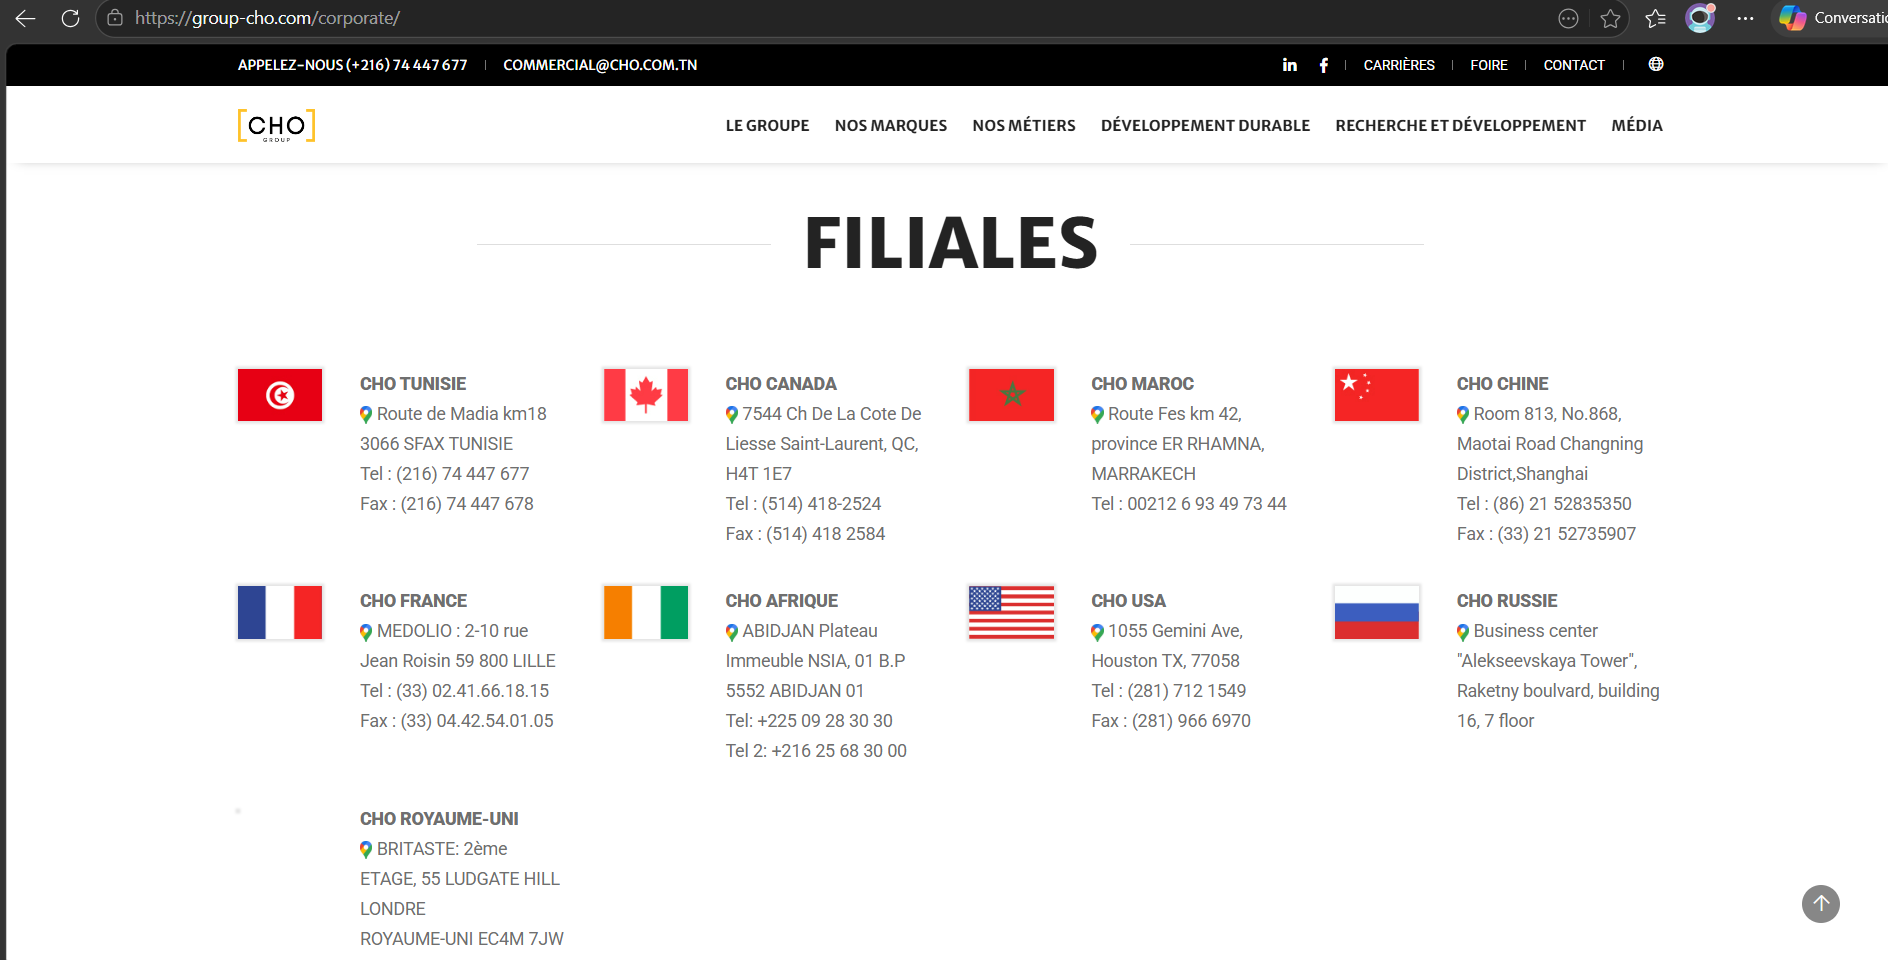
\includegraphics[width=0.90\textwidth]{Filiales.png}
\caption{Présence internationale de CHO Group}
\label{fig:cho_filiales_ch1}
\end{figure}

Cette dimension internationale implique une forte exposition à la concurrence ainsi qu'à la variabilité des prix, ce qui rend le suivi des marchés particulièrement stratégique pour l'entreprise.

\section{Activités de l'entreprise}

Les activités principales de CHO Group couvrent l'ensemble du processus de production et de distribution :

\begin{itemize}[leftmargin=1.2cm]
	\item production d'huile d'olive ;
	\item raffinage et transformation ;
	\item conditionnement ;
	\item exportation vers plusieurs marchés internationaux.
\end{itemize}

\begin{figure}[H]
\centering
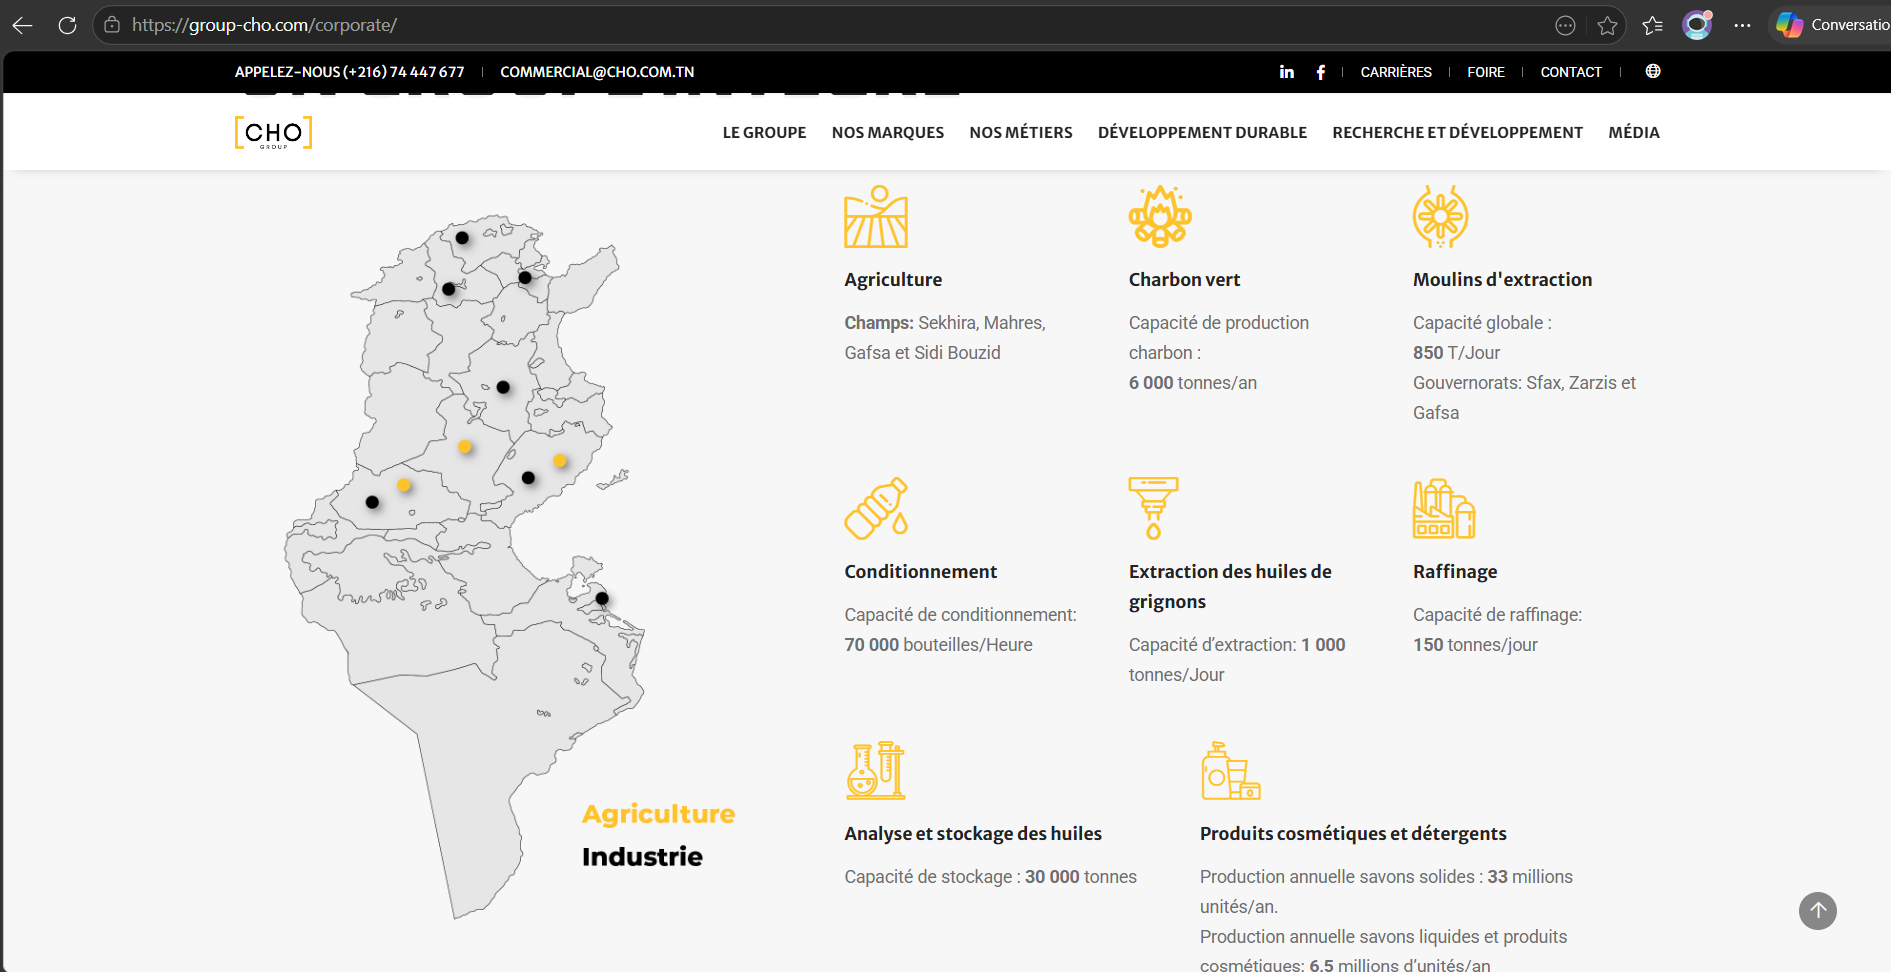
\includegraphics[width=0.90\textwidth]{un_group_integre.png}
\caption{Chaîne de valeur et processus intégré de CHO Group}
\label{fig:cho_integre_ch1}
\end{figure}

Ces activités impliquent la gestion de marchés multiples et nécessitent un suivi rigoureux des prix afin de maintenir la compétitivité et optimiser les décisions commerciales.

\section{Étude de l'existant}

Avant la mise en place de ce projet, le processus de suivi des prix au sein de l'entreprise reposait principalement sur des méthodes manuelles.

Dans un premier temps, les équipes se déplacent vers les points de vente (marchés, magasins, grandes surfaces) afin de collecter les prix des produits. En parallèle, certaines données peuvent être récupérées à partir de sources en ligne selon les besoins.

\begin{figure}[H]
\centering
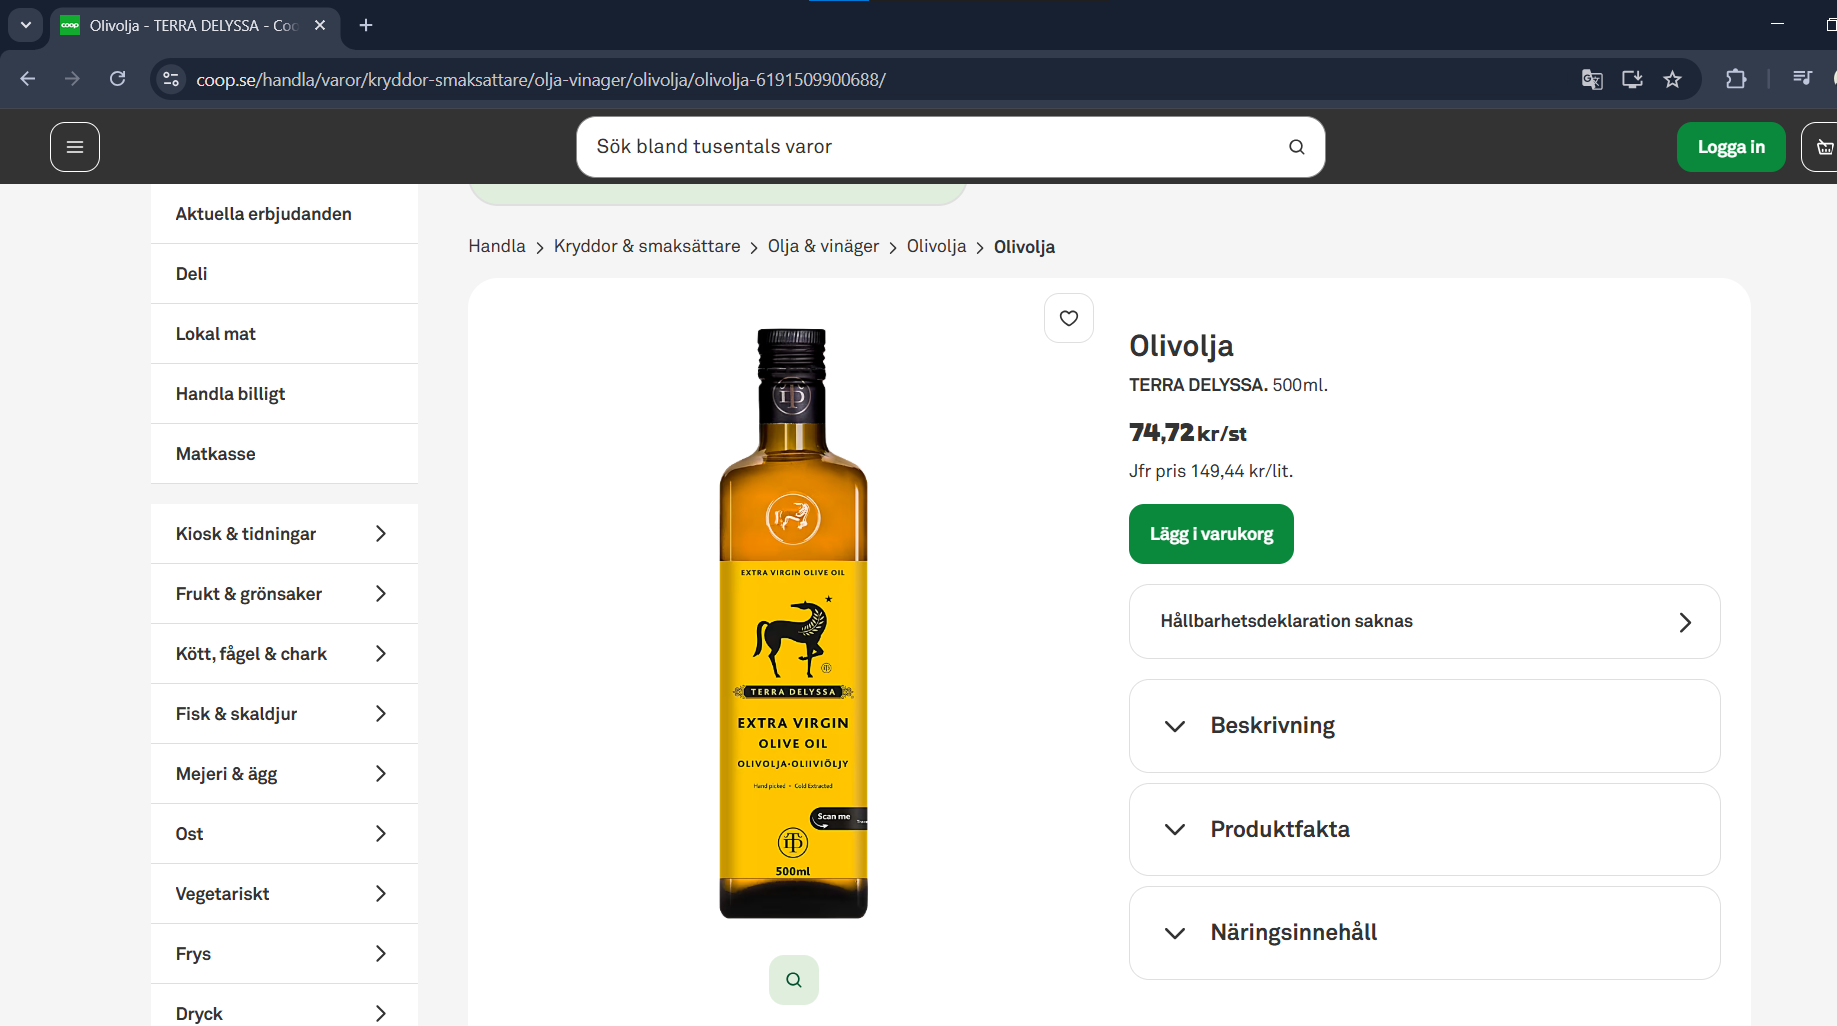
\includegraphics[width=0.92\textwidth]{example_source_of_data.png}
\caption{Exemple de source de données utilisée pour la collecte des prix}
\label{fig:source_donnees_ch1}
\end{figure}

Dans un second temps, les données collectées sont saisies manuellement dans des fichiers Excel.

\begin{figure}[H]
\centering
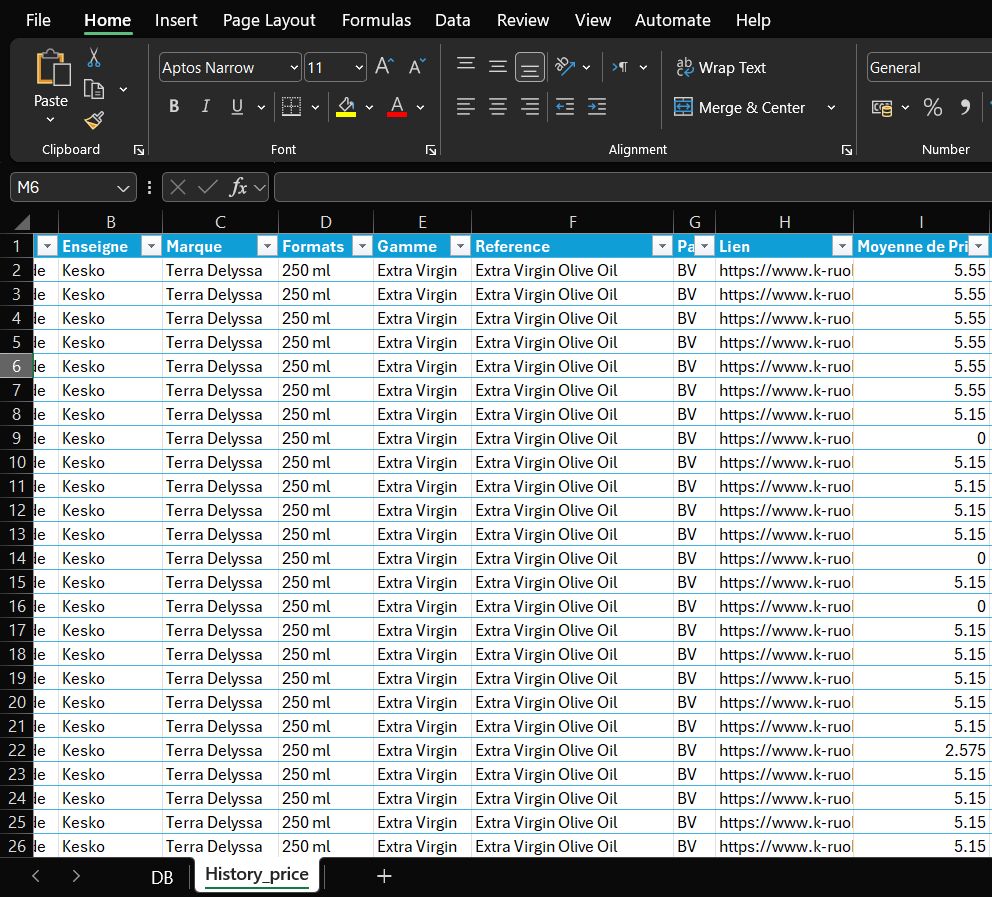
\includegraphics[width=0.92\textwidth]{Excel_image_example.png}
\caption{Exemple de fichier Excel utilisé dans le processus actuel}
\label{fig:excel_existant_ch1}
\end{figure}

Enfin, les opérations de tri, de nettoyage et d'analyse sont réalisées manuellement, ce qui rend le processus long et dépendant des interventions humaines.

Le processus global peut être résumé comme suit :

\begin{itemize}[leftmargin=1.2cm]
	\item collecte terrain et/ou web ;
	\item saisie manuelle des données ;
	\item traitement et analyse manuelle.
\end{itemize}

\begin{figure}[H]
\centering
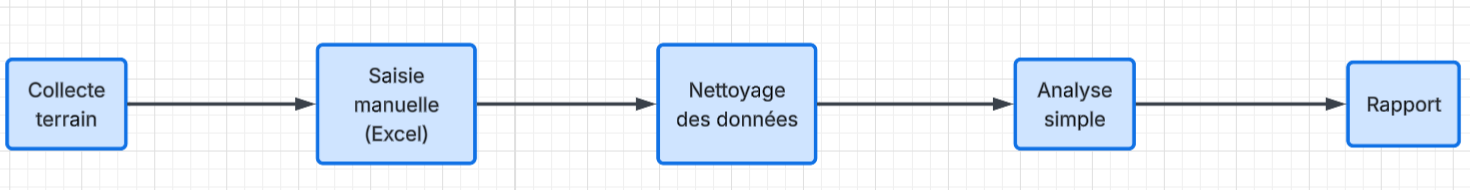
\includegraphics[width=0.92\textwidth]{old_company_solution.png}
\caption{Schéma du système actuel : collecte, Excel et analyse manuelle}
\label{fig:process_actuel_ch1}
\end{figure}

\section{Critique de l'existant}

L'analyse du système actuel met en évidence plusieurs limites importantes :

\begin{itemize}[leftmargin=1.2cm]
	\item un processus lent, dû à la collecte manuelle et aux traitements non automatisés ;
	\item un risque élevé d'erreurs lors de la saisie des données ;
	\item une difficulté d'accès rapide à une information fiable et consolidée ;
	\item une absence de vision globale et en temps réel des prix ;
	\item une forte dépendance au travail humain.
\end{itemize}

Ces contraintes impactent directement la qualité et la rapidité de la prise de décision au sein de l'entreprise.

\section{Objectifs du projet}

Afin de répondre aux limites identifiées, ce projet a pour objectif de mettre en place une solution de Business Intelligence permettant :

\begin{itemize}[leftmargin=1.2cm]
	\item d'automatiser la collecte des données à partir de différentes sources ;
	\item de centraliser les données dans une base unique ;
	\item d'améliorer la qualité et la fiabilité des données ;
	\item de produire des indicateurs clés (KPI) pour le pilotage ;
	\item de fournir des tableaux de bord interactifs pour l'analyse.
\end{itemize}

Ce projet se concentre sur une approche descriptive et analytique, constituant une base solide pour de futures évolutions vers des analyses plus avancées.

\section{Solution proposée}

La solution proposée consiste en une plateforme de Business Intelligence permettant de transformer un processus manuel en un système automatisé et structuré.

Elle repose sur plusieurs composants principaux :

\begin{itemize}[leftmargin=1.2cm]
	\item des sources de données (web et terrain) ;
	\item un processus ETL pour la collecte et le traitement ;
	\item une base de données centralisée ;
	\item une interface de visualisation sous forme de tableaux de bord.
\end{itemize}

\begin{figure}[H]
\centering
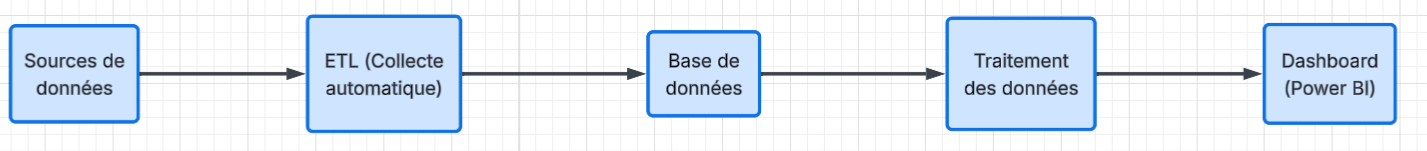
\includegraphics[width=0.92\textwidth]{our_diagram_solution.png}
\caption{Schéma de la solution BI : sources, ETL, base de données et dashboard}
\label{fig:solution_bi_ch1}
\end{figure}

Cette solution permet de réduire l'intervention manuelle, d'améliorer la fiabilité des données et de fournir une vision claire et exploitable des prix, facilitant ainsi la prise de décision.

\section{Conclusion}

Ce chapitre a permis de présenter le contexte général de l'entreprise ainsi que le fonctionnement du système actuel. L'analyse de l'existant a mis en évidence plusieurs limites justifiant la mise en place d'une solution de Business Intelligence adaptée.

Le chapitre suivant sera consacré à l'analyse des besoins et à la conception de la solution proposée.

\clearpage

\chapter{Analyse et conception}

\section{Introduction}
Ce chapitre formalise les besoins du projet puis presente la conception fonctionnelle et technique de \ProjectName. L'objectif est de traduire la problematique metier en un systeme coherent, evolutif et securise.

\section{Specification des besoins}
\subsection{Acteurs}
Deux acteurs principaux sont identifies :
\begin{itemize}[leftmargin=1.2cm]
	\item \textbf{Administrateur technique} : gere le catalogue, les URLs, les utilisateurs et la supervision operationnelle.
	\item \textbf{Analyste metier} : consulte les indicateurs, compare les prix et interprete les tendances.
\end{itemize}

\subsection{Besoins fonctionnels}
Les besoins fonctionnels retenus sont :
\begin{itemize}[leftmargin=1.2cm]
	\item extraction automatisee des prix depuis les sites cibles ;
	\item transformation et nettoyage des donnees (ETL) ;
	\item historisation hebdomadaire et normalisation en EUR ;
	\item visualisation interactive des prix et tendances ;
	\item comparaison par pays, enseigne et magasin ;
	\item administration complete (produits, URLs, utilisateurs) ;
	\item suivi de la qualite de collecte (Operational Visibility).
\end{itemize}

\subsection{Besoins non fonctionnels}
\begin{itemize}[leftmargin=1.2cm]
	\item \textbf{Fiabilite} : controles de validite sur les donnees entrantes.
	\item \textbf{Securite} : authentification et controle des acces par role.
	\item \textbf{Performance} : temps de reponse acceptable pour un usage quotidien.
	\item \textbf{Scalabilite} : possibilite d'ajouter de nouveaux pays et nouveaux sites.
	\item \textbf{Maintenabilite} : architecture modulaire et claire.
\end{itemize}

\section{Analyse conceptuelle (UML)}
\subsection{Diagramme de cas d'utilisation}
Le diagramme de cas d'utilisation met en evidence les interactions entre les deux acteurs et les fonctions principales de la plateforme.

\figureplaceholder{Diagramme UML de cas d'utilisation (Admin technique / Analyste metier)}{Cas d'utilisation principaux de \ProjectName}

\subsection{Diagramme de sequence}
Le diagramme de sequence principal represente le flux de donnees de bout en bout : source web -> scraping -> ETL -> base PostgreSQL -> API FastAPI -> interface React.

\figureplaceholder{Diagramme UML de sequence du flux de donnees}{Sequence globale de traitement et de consultation}

\section{Conception de la base de donnees}
\subsection{Dictionnaire de donnees (extrait)}
\begin{table}[H]
\centering
\caption{Extrait du dictionnaire de donnees}
\begin{tabular}{p{3.5cm}p{4.0cm}p{5.9cm}}
\toprule
\textbf{Entite} & \textbf{Attribut cle} & \textbf{Description} \\
\midrule
product\_formats & product\_format\_id & variante produit (brand/category/range/format/packaging) \\
product\_urls & url, is\_active & source de scraping associee a un produit/site/magasin \\
raw\_staging & payload, status, scraped\_at & donnees brutes collecte + etat de traitement \\
weekly\_price\_summary & week\_start, avg\_price, currency & consolidation hebdomadaire exploitee par le dashboard \\
\bottomrule
\end{tabular}
\end{table}

\subsection{Modele logique de donnees (MLD)}
La conception adopte une separation claire entre :
\begin{itemize}[leftmargin=1.2cm]
	\item donnees de reference (catalogue, sites, magasins) ;
	\item donnees brutes de collecte ;
	\item donnees nettoyees et analytiques.
\end{itemize}

\figureplaceholder{Modele logique de donnees (MLD) du projet}{Schema logique de la base PostgreSQL}

\subsection{Regles de conception}
\begin{itemize}[leftmargin=1.2cm]
	\item cles etrangeres pour garantir la coherence relationnelle ;
	\item contraintes d'unicite sur les combinaisons critiques ;
	\item index sur les colonnes de recherche frequente ;
	\item regles de qualite (exclusion des prix <= 0).
\end{itemize}

\section{Architecture logique de la solution}
La solution est concue en couches : collecte, ETL, stockage, API, presentation. Cette decomposition permet d'isoler les responsabilites et de simplifier la maintenance.

\figureplaceholder{Architecture logique en couches}{Conception modulaire de \ProjectName}

\section{Conclusion}
L'analyse et la conception realisent le lien entre besoins metier et implementation technique. Elles fournissent une base robuste pour une realisation progressive et maitrisee de la plateforme.

\clearpage

\chapter{Realisation et implementation}

\section{Introduction}
Ce chapitre decrit la mise en oeuvre technique de \ProjectName, depuis l'architecture logicielle jusqu'aux interfaces utilisateur exploitees par les equipes metier.

\section{Architecture technique de la solution}
La solution realisee s'appuie sur une architecture full-stack data orientee services.

\begin{table}[H]
\centering
\caption{Stack technique de \ProjectName}
\begin{tabular}{p{3.8cm}p{9.2cm}}
\toprule
\textbf{Couche} & \textbf{Technologies} \\
\midrule
Collecte & Python, Playwright, parseurs par site \\
Traitement & Python, Pandas, ETL hebdomadaire \\
Stockage & PostgreSQL \\
Services API & FastAPI, Pydantic, JWT \\
Interface & React, Vite, TypeScript, TanStack Query \\
\bottomrule
\end{tabular}
\end{table}

\figureplaceholder{Diagramme d'architecture technique complete}{Architecture technique de la plateforme}

\section{Collecte et transformation des donnees (Pipeline ETL)}
\subsection{Scraping automatise}
La collecte des prix est automatisee via des scrapers dedies aux sites cibles selon les priorites commerciales. Les donnees brutes sont stockees dans \texttt{raw\_staging} avec statut, code HTTP et capture d'ecran.

\subsection{Traitements ETL}
Le pipeline ETL nettoie les donnees, convertit les formats et consolide les prix dans les tables analytiques.

\begin{itemize}[leftmargin=1.2cm]
	\item validation des montants ;
	\item rejet des valeurs invalides (<= 0) ;
	\item normalisation des devises vers EUR ;
	\item calcul des agrégats hebdomadaires.
\end{itemize}

\begin{lstlisting}[language=Python,caption={Orchestration simplifiee du pipeline principal}]
if __name__ == "__main__":
    fetch_and_store_exchange_rates()
    run_all_scrapers()
    run_etl()
\end{lstlisting}

\figureplaceholder{Capture d'execution du pipeline en terminal}{Execution end-to-end du pipeline}

\section{Backend API et securite}
Le backend FastAPI expose les endpoints necessaires au dashboard : prix, filtres, series temporelles, administration et supervision operationnelle.

La securite est assuree par authentification token et controle d'acces base sur les roles :
\begin{itemize}[leftmargin=1.2cm]
	\item \textbf{admin} : acces complet y compris configuration ;
	\item \textbf{user} : consultation analytique.
\end{itemize}

\figureplaceholder{Capture API docs / endpoints principaux}{Services exposes par FastAPI}

\section{Presentation des interfaces}
\subsection{Vues analytiques}
\begin{itemize}[leftmargin=1.2cm]
	\item \textbf{Prices Explorer} : exploration detaillee des prix avec filtre et source URL.
	\item \textbf{Price Trends} : evolution hebdomadaire des prix normalises.
	\item \textbf{Store Comparison} : comparaison concurrentielle par enseigne/magasin.
\end{itemize}

\subsection{Vues administratives}
\begin{itemize}[leftmargin=1.2cm]
	\item gestion du catalogue produits (brands/categories/ranges/formats) ;
	\item gestion des URLs de collecte ;
	\item matrice Retail Presence ;
	\item supervision des echecs (Operational Visibility) ;
	\item gestion des utilisateurs.
\end{itemize}

\figureplaceholder{Capture dashboard principal}{Vue globale de l'interface}
\figureplaceholder{Capture page Retail Presence}{Pilotage de la couverture produit}
\figureplaceholder{Capture page Operational Visibility}{Supervision des incidents de collecte}

\section{Mise en oeuvre pratique}
L'exploitation de la plateforme suit cinq etapes :
\begin{enumerate}[leftmargin=1.2cm]
	\item preparation de l'environnement Python et installation des dependances ;
	\item initialisation de la base PostgreSQL ;
	\item chargement des donnees initiales ;
	\item execution du pipeline ;
	\item lancement backend et frontend.
\end{enumerate}

\section{Contributions des etudiants}
Le projet a ete realise en co-construction par \textbf{Khalil Amamri} et \textbf{Mahdi ElhadjAmor}, avec une implication sur la conception, l'implementation et la validation.

\section{Conclusion}
La phase de realisation confirme la faisabilite et la valeur operationnelle de \ProjectName. Le systeme relie des donnees web heterogenes a des indicateurs decisionnels directement exploitables par l'entreprise.

\clearpage

\chapter*{Conclusion generale}
\addcontentsline{toc}{chapter}{Conclusion generale}

Ce projet de fin d'etudes avait pour ambition de transformer un besoin metier concret en une solution numerique complete. L'objectif a ete atteint avec la realisation de \textbf{\ProjectOfficialTitle}, ci-apres \textbf{\ProjectName}, une plateforme integree de veille des prix internationaux, allant de la collecte web jusqu'a la visualisation decisionnelle.

\section*{Bilan des apports}
Les principaux apports du projet sont :
\begin{itemize}[leftmargin=1.2cm]
	\item automatisation d'un processus historiquement lourd et partiellement manuel ;
	\item centralisation des donnees prix dans un modele relationnel fiable ;
	\item normalisation des prix en EUR pour des comparaisons internationales ;
	\item disponibilite d'un dashboard professionnel pour les profils metier et admin.
\end{itemize}

\section*{Contribution des etudiants}
Le projet valorise une collaboration reelle entre \textbf{Khalil Amamri} et \textbf{Mahdi ElhadjAmor}, avec une implication continue sur la conception, l'implementation et la validation. Cette dynamique d'equipe a permis d'assurer la coherence de la solution de bout en bout.

\section*{Impact pour l'entreprise}
Pour CHO, la plateforme apporte une meilleure visibilite sur les prix, une reduction du temps d'analyse et une meilleure capacite de pilotage des decisions commerciales dans un environnement international.

\section*{Perspectives}
Les perspectives naturelles d'evolution sont :
\begin{itemize}[leftmargin=1.2cm]
	\item integration de nouveaux pays, enseignes et familles de produits ;
	\item mise en place d'alertes automatiques (variation forte, absence de donnees, anomalies) ;
	\item industrialisation des tests automatiques et deploiement CI/CD.
\end{itemize}

En conclusion, \ProjectName{} constitue une base solide et evolutive pour la veille strategique des prix, avec une valeur immediate pour les utilisateurs et un potentiel important pour les futures iterations.

\clearpage

\chapter*{Bibliographie}
\addcontentsline{toc}{chapter}{Bibliographie}

\begin{enumerate}[leftmargin=1.2cm]
	\item CHO Group, \textit{Corporate - Le Groupe}, consulte en avril 2026. \url{https://group-cho.com/corporate/}
	\item CHO Group, \textit{Corporate - CHO Group en chiffres}, consulte en avril 2026. \url{https://group-cho.com/corporate/}
	\item CHO Group, \textit{Corporate - Filiales}, consulte en avril 2026. \url{https://group-cho.com/corporate/}
	\item CHO Group, \textit{Corporate - Groupe integre / Nos metiers}, consulte en avril 2026. \url{https://group-cho.com/corporate/}
	\item FastAPI Documentation, \textit{FastAPI Framework}, consulte en 2026. \url{https://fastapi.tiangolo.com/}
	\item PostgreSQL Global Development Group, \textit{PostgreSQL Documentation}, consulte en 2026. \url{https://www.postgresql.org/docs/}
	\item React Team, \textit{React Documentation}, consulte en 2026. \url{https://react.dev/}
	\item Vite Team, \textit{Vite Guide}, consulte en 2026. \url{https://vitejs.dev/guide/}
	\item Microsoft, \textit{Playwright Documentation}, consulte en 2026. \url{https://playwright.dev/}
	\item TanStack, \textit{TanStack Query Documentation}, consulte en 2026. \url{https://tanstack.com/query/latest}
\end{enumerate}

\clearpage

\appendix
\chapter{Annexes}

\section{Annexe A - Captures institutionnelles CHO Group (selection essentielle)}
\begin{figure}[H]
\centering
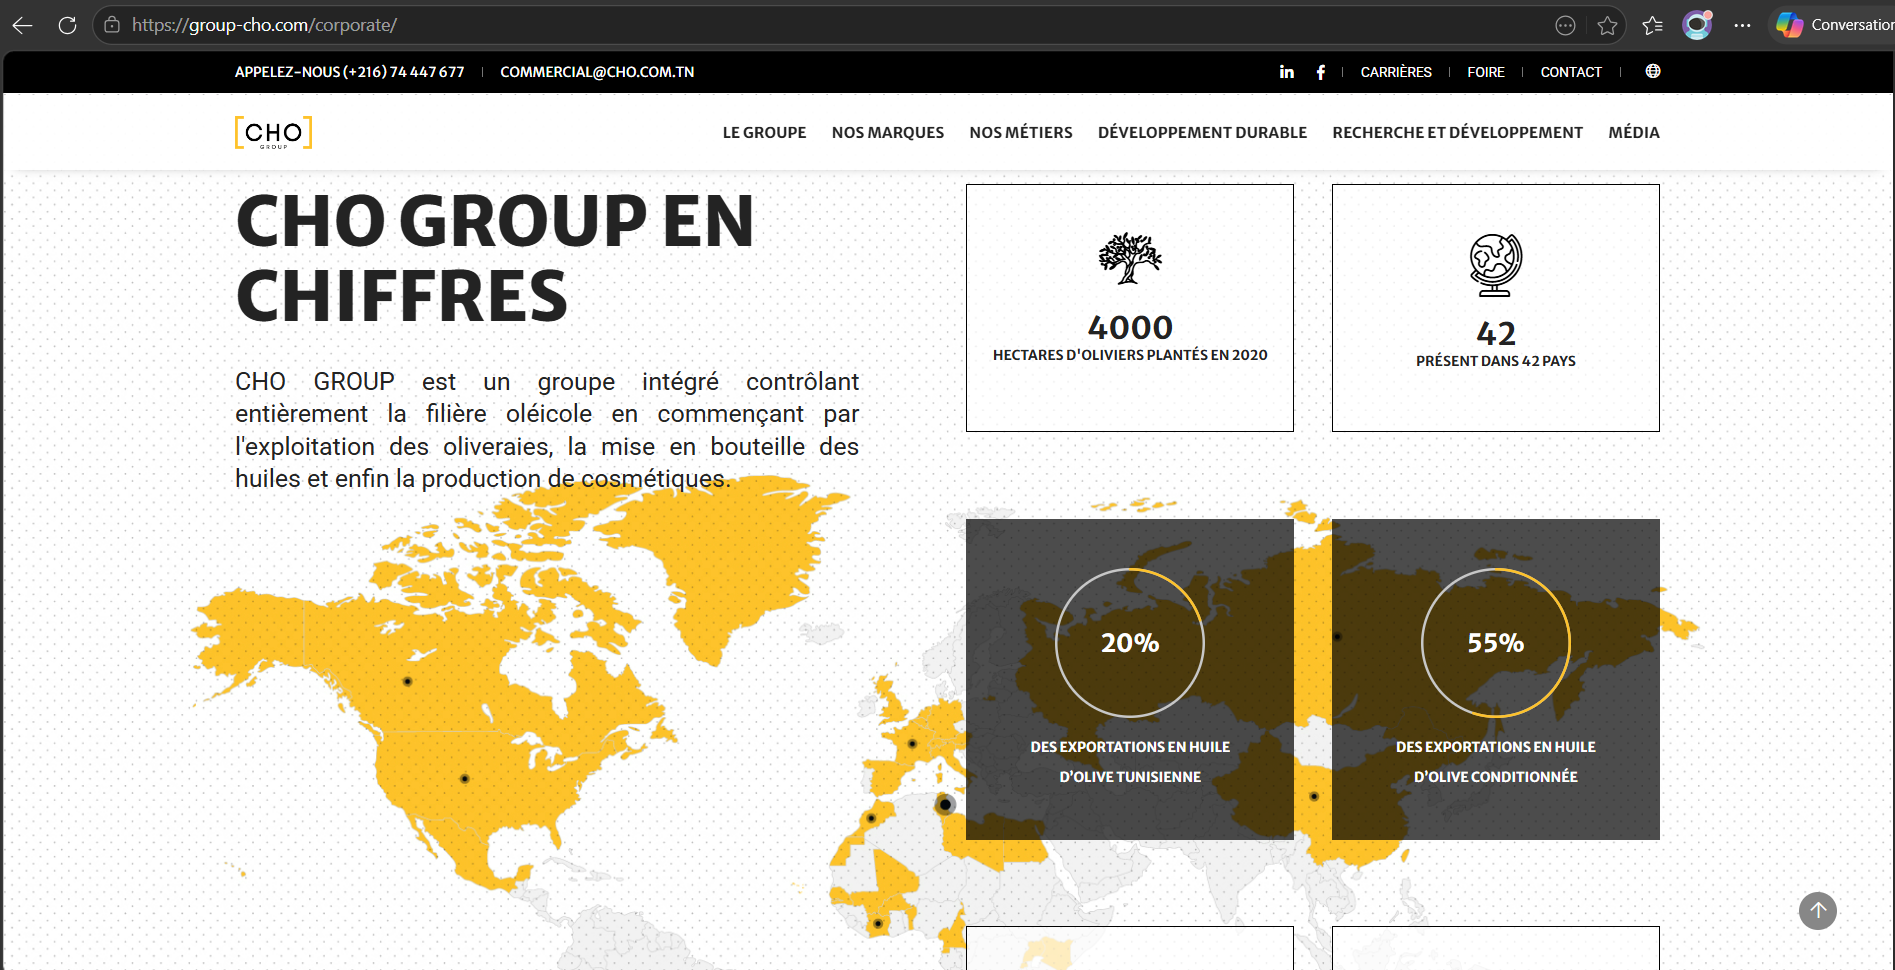
\includegraphics[width=0.90\textwidth]{cho_group_en_chiffres.png}
\caption{CHO Group en chiffres : indicateurs de dimension internationale}
\end{figure}

\begin{figure}[H]
\centering
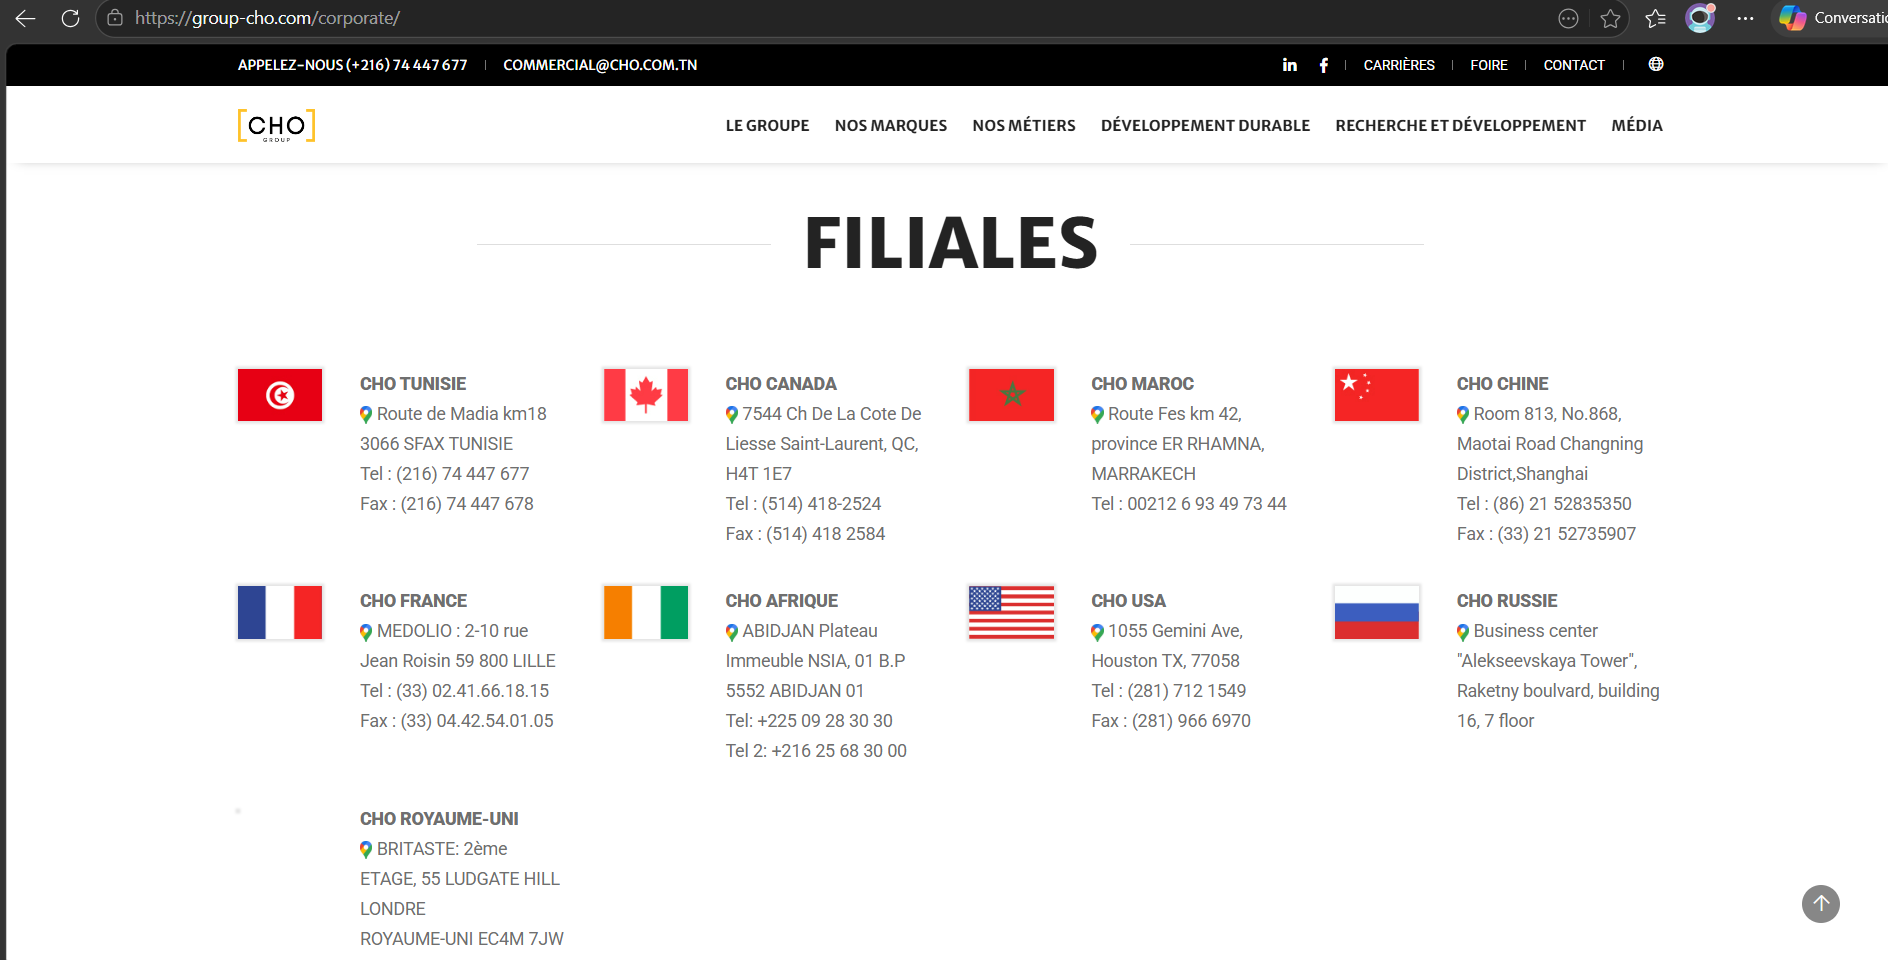
\includegraphics[width=0.90\textwidth]{Filiales.png}
\caption{Filiales CHO Group : couverture internationale}
\end{figure}

\begin{figure}[H]
\centering
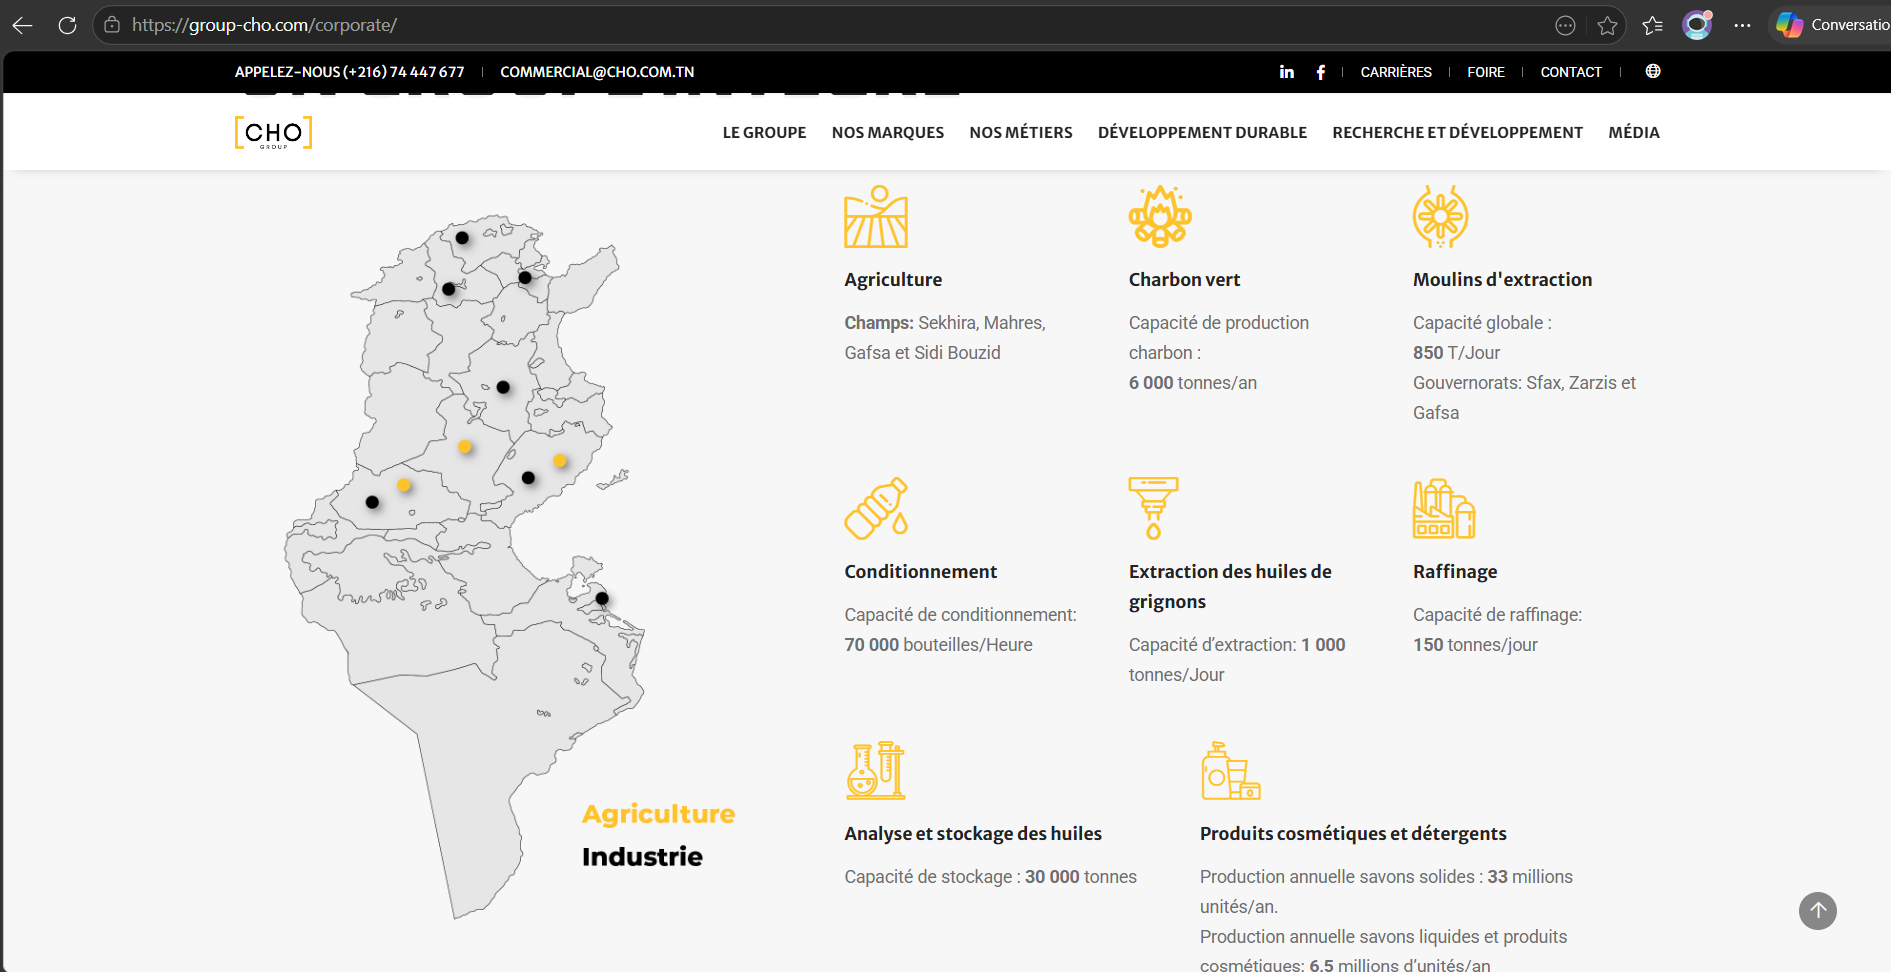
\includegraphics[width=0.90\textwidth]{un_group_integre.png}
\caption{CHO Group integre : activites et chaine de valeur}
\end{figure}

\section{Annexe B - Diagrammes techniques}
\figureplaceholder{Diagramme ERD final exporte depuis l'outil de modelisation}{Modele de donnees detaille}
\figureplaceholder{Diagramme d'architecture de deploiement}{Architecture de deploiement}
\figureplaceholder{Diagramme de sequence du pipeline}{Sequence de traitement quotidienne}

\section{Annexe C - Indicateurs metier de reference}
\begin{table}[H]
\centering
\caption{Exemples d'indicateurs suivis par la direction}
\begin{tabular}{p{4.3cm}p{4.6cm}p{4.4cm}}
\toprule
\textbf{Indicateur} & \textbf{Finalite} & \textbf{Periodicite} \\
\midrule
Prix moyen par marche & Mesurer la competitivite prix & Hebdomadaire \\
Variation vs semaine N-1 & Detecter une baisse/hausse critique & Hebdomadaire \\
Couverture Retail Presence & Identifier les manques de visibilite & Hebdomadaire \\
Taux d'echec de collecte & Piloter la fiabilite data & Quotidienne \\
\bottomrule
\end{tabular}
\end{table}

\section{Annexe D - Scenarios de decision commerciale}
\begin{table}[H]
\centering
\caption{Exemples de scenarios de pilotage}
\begin{tabular}{p{4.1cm}p{4.9cm}p{4.3cm}}
\toprule
\textbf{Situation observee} & \textbf{Decision possible} & \textbf{Effet attendu} \\
\midrule
Baisse rapide d'un concurrent sur un marche cle & Ajustement prix/promo court terme & Reduction de la perte de volume \\
Hausse structurelle sur un marche & Repositionnement progressif & Preservation de la marge \\
Faible couverture produit sur une enseigne & Priorisation des URLs et formats & Meilleure visibilite concurrentielle \\
\bottomrule
\end{tabular}
\end{table}

\section{Annexe E - Plan de remplissage des figures}
Le rapport retient prioritairement les captures qui renforcent la justification metier du projet : presence internationale, chiffres cles et chaine de valeur. Le dossier \texttt{reports/figures} centralise les visuels utilises.

\clearpage


\end{document}
